% Required packages: graphicx, booktabs, longtable, array, pdflscape.
% Compile the parent manuscript with XeLaTeX or LuaLaTeX because the original queries are multilingual.
\section{Visual Skill Selection and Application}
\label{app:skill_selection_application}

We present 16 qualitative cases of Visual Skill selection and application. For each case, we report the selected Skills and compare websites generated by Claude Opus 5 under three settings: No Skill, General Website Design Skill, and Website-Derived Visual Skill. These cases demonstrate the selection and application of Visual Skills; they are separate from the distilled-model results presented later.

\begin{landscape}
\begingroup
\footnotesize
\setlength{\tabcolsep}{5pt}
\renewcommand{\arraystretch}{1.12}
\begin{longtable}{>{\raggedright\arraybackslash}p{0.61\linewidth} >{\raggedright\arraybackslash}p{0.35\linewidth}}
\caption{Visual Skill selection and application by Claude Opus 5. Each case reports the original query and selected Website-Derived Visual Skill(s), followed by homepage renderings under the No Skill, General Website Design Skill, and Website-Derived Visual Skill conditions.}
\label{tab:visual_skill_selection_application}\\
\toprule
\textbf{Query} & \textbf{Skill Selection} \\
\midrule
\endfirsthead
\multicolumn{2}{l}{\footnotesize\itshape Continued from the previous page}\\
\toprule
\textbf{Query} & \textbf{Skill Selection} \\
\midrule
\endhead
\midrule
\multicolumn{2}{r}{\footnotesize\itshape Continued on the next page}\\
\endfoot
\bottomrule
\endlastfoot
\textbf{Case 01: World Cup Live Experience}\par\smallskip Para criar uma página de promoção da copa do mundo, é necessário incluir tabela de pontos em tempo real, condições de guerra em tempo real, reprodução maravilhosa e assim por diante, os problemas de detalhes me ajudam a considerar a melhoria; & \texttt{split\_\allowbreak{}flap\_\allowbreak{}live\_\allowbreak{}value\_\allowbreak{}board}\par\emph{Stock Ticker Dashboard}\medskip\par \texttt{center\_\allowbreak{}locked\_\allowbreak{}media\_\allowbreak{}row\_\allowbreak{}over\_\allowbreak{}live\_\allowbreak{}backdrop}\par\emph{Orken}\medskip\par \texttt{aperture\_\allowbreak{}framed\_\allowbreak{}scroll\_\allowbreak{}scrubbed\_\allowbreak{}clip}\par\emph{Scroll-Synced Video with Timed Cues and Keyhole Effect} \\*
\addlinespace[4pt]
\multicolumn{2}{c}{\begin{minipage}[t]{0.318\linewidth}\centering \textbf{No Skill}\\[3pt]
\includegraphics[width=\linewidth]{screenshots/pdf/world-cup/no_skill.pdf}\end{minipage}\hfill \begin{minipage}[t]{0.318\linewidth}\centering \textbf{General Website Design Skill}\\[3pt]
\includegraphics[width=\linewidth]{screenshots/pdf/world-cup/general_skill.pdf}\end{minipage}\hfill \begin{minipage}[t]{0.318\linewidth}\centering \textbf{Website-Derived Visual Skill}\\[3pt]
\includegraphics[width=\linewidth]{screenshots/pdf/world-cup/visual_skill.pdf}\end{minipage}} \\
\addlinespace[7pt]\midrule
\textbf{Case 02: Marketing Course Landing Page}\par\smallskip Create a marketing course introduction page, including a list of courses and sub-courses, along with some course demonstrations and the results achieved by the students； & \texttt{center\_\allowbreak{}out\_\allowbreak{}photo\_\allowbreak{}bloom\_\allowbreak{}with\_\allowbreak{}pointer\_\allowbreak{}drift}\par\emph{How to Create a Motion Hover Effect for a Background Image Grid} \\*
\addlinespace[4pt]
\multicolumn{2}{c}{\begin{minipage}[t]{0.318\linewidth}\centering \textbf{No Skill}\\[3pt]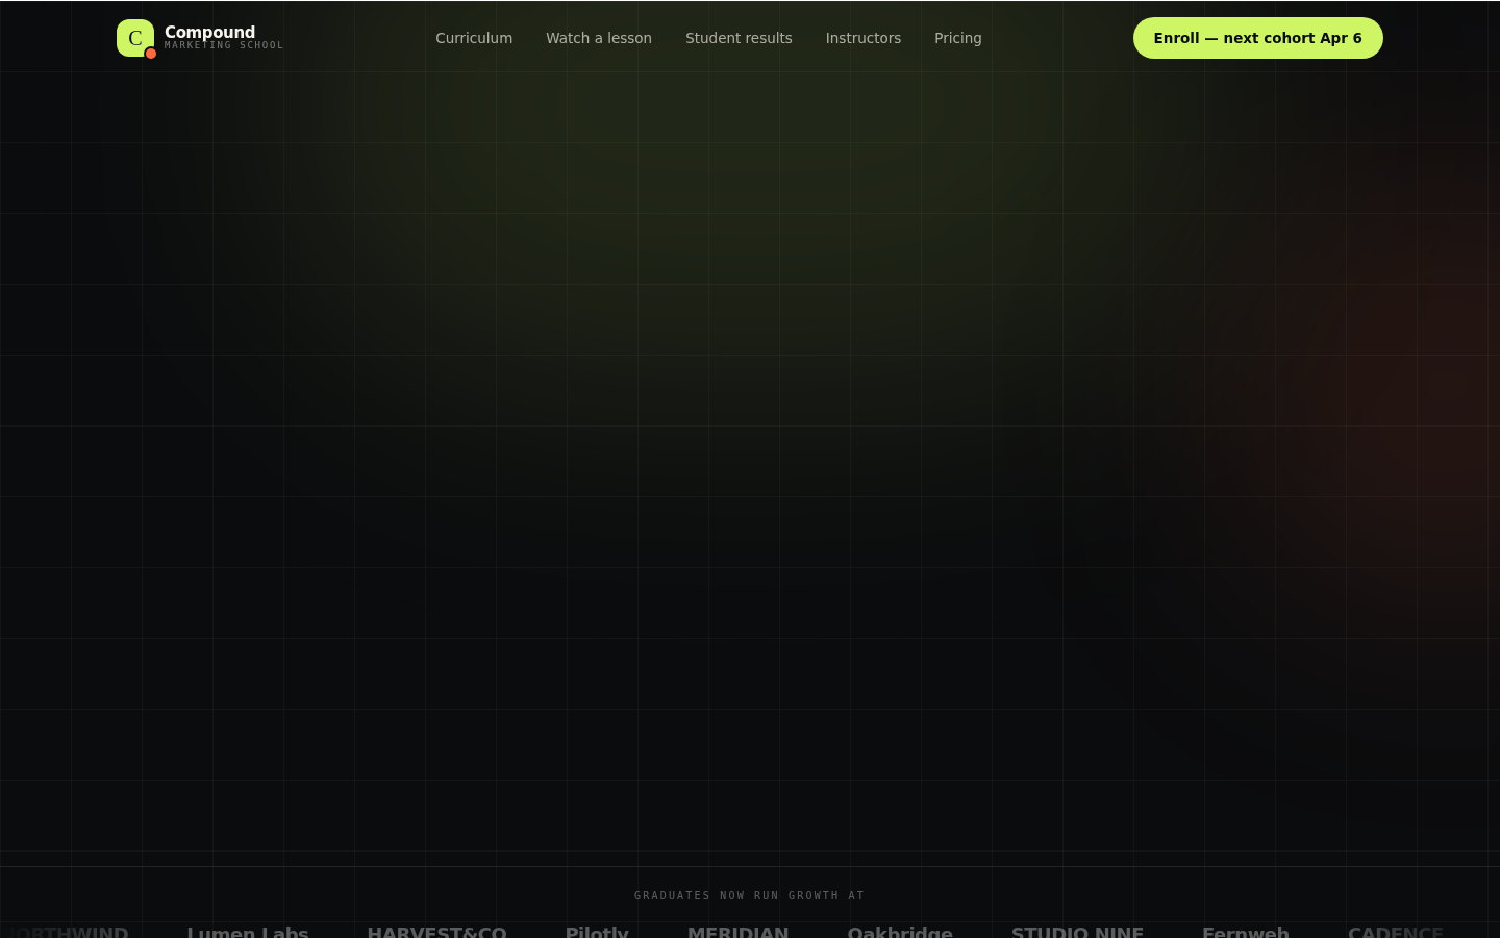
\includegraphics[width=\linewidth]{screenshots/pdf/p-03/no_skill.pdf}\end{minipage}\hfill \begin{minipage}[t]{0.318\linewidth}\centering \textbf{General Website Design Skill}\\[3pt]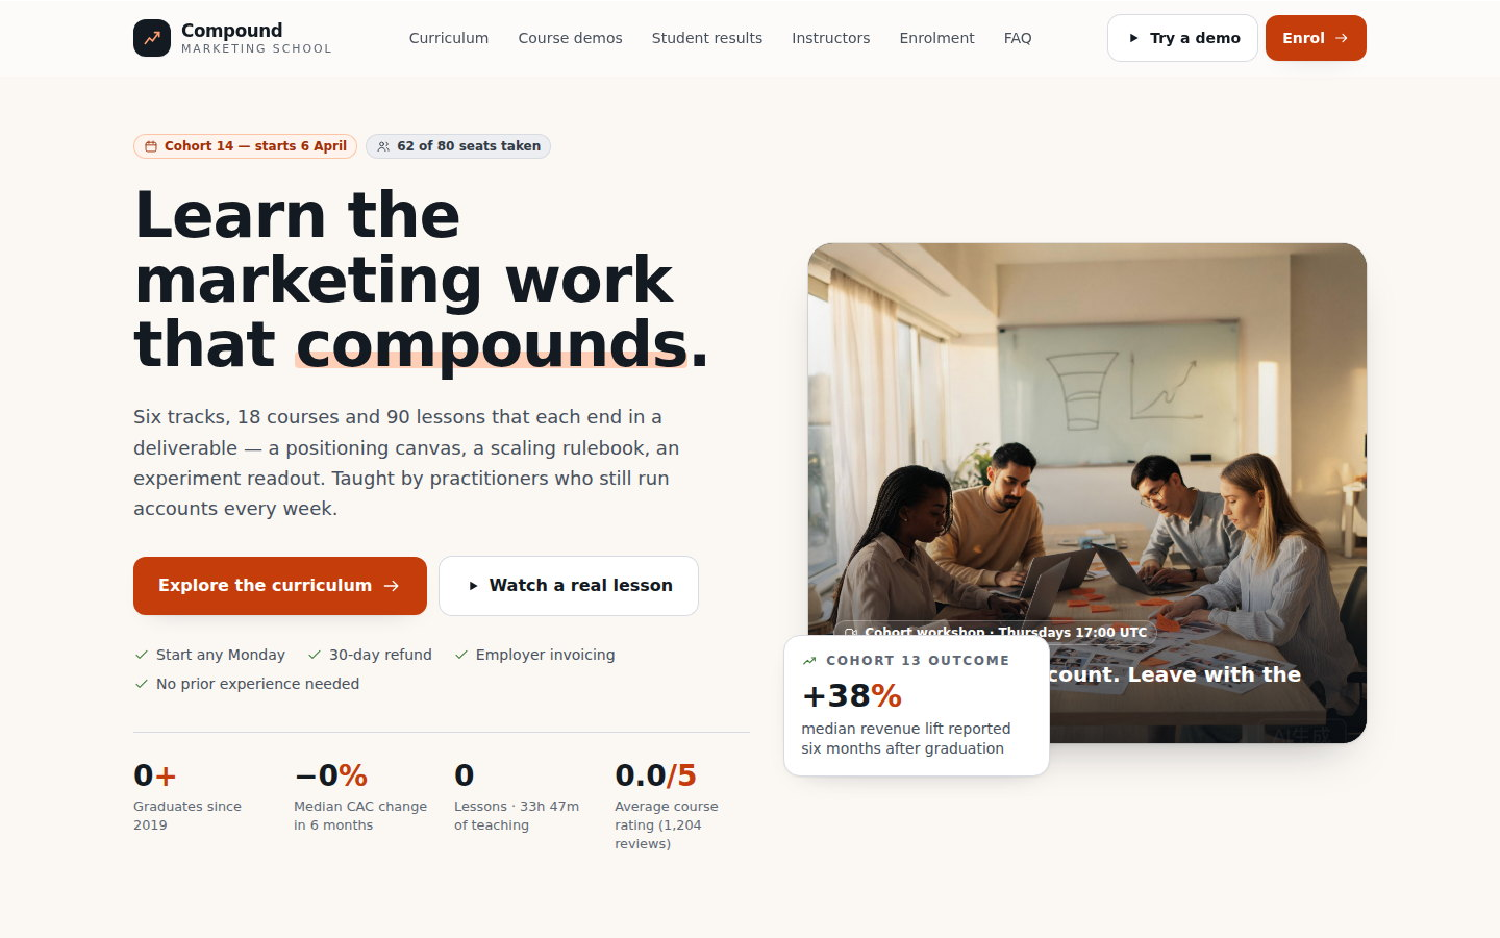
\includegraphics[width=\linewidth]{screenshots/pdf/p-03/general_skill.pdf}\end{minipage}\hfill \begin{minipage}[t]{0.318\linewidth}\centering \textbf{Website-Derived Visual Skill}\\[3pt]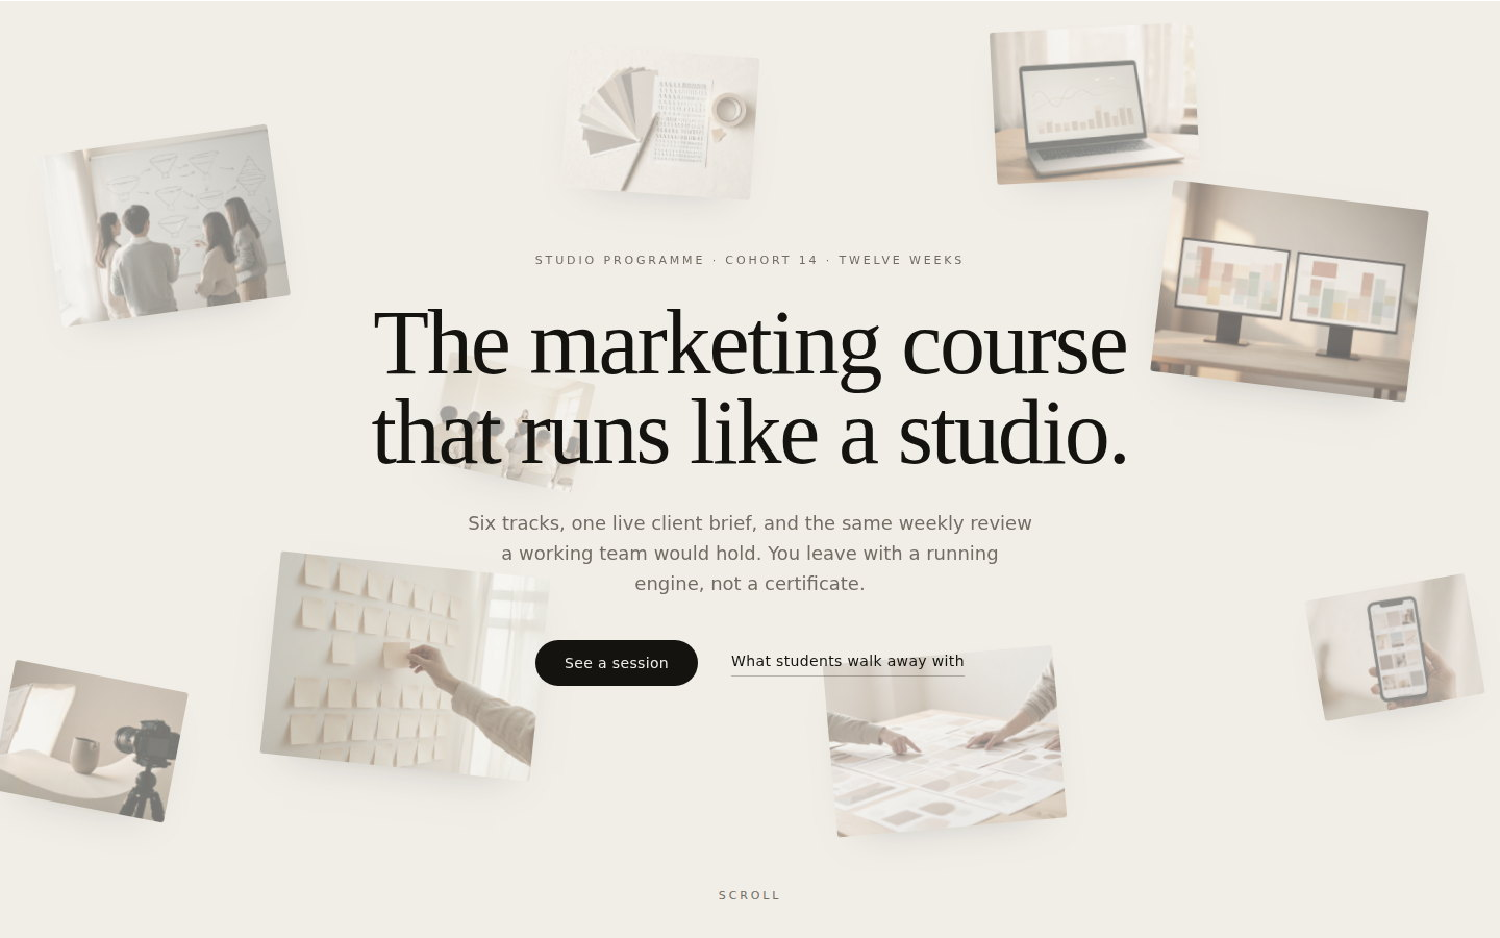
\includegraphics[width=\linewidth]{screenshots/pdf/p-03/visual_skill.pdf}\end{minipage}} \\
\addlinespace[7pt]\midrule
\textbf{Case 03: Premium Auto Parts}\par\smallskip Ich möchte eine offizielle Website für eine Marke von Autoteilen erstellen, die den minimalistischen Designstil der Apple-Website aufgreift, um die Professionalität und hochwertige Qualität der Autoteile zu unterstreichen und Besuchern einen direkten Eindruck von der technologischen Leistung und dem Handwerksstandard der Produkte zu vermitteln. & \texttt{scroll\_\allowbreak{}scrubbed\_\allowbreak{}object\_\allowbreak{}opening\_\allowbreak{}walkthrough}\par\emph{Apple-Style Scroll Animation  3D Product Explode} \\*
\addlinespace[4pt]
\multicolumn{2}{c}{\begin{minipage}[t]{0.318\linewidth}\centering \textbf{No Skill}\\[3pt]
\includegraphics[width=\linewidth]{screenshots/pdf/p-06/no_skill.pdf}\end{minipage}\hfill \begin{minipage}[t]{0.318\linewidth}\centering \textbf{General Website Design Skill}\\[3pt]
\includegraphics[width=\linewidth]{screenshots/pdf/p-06/general_skill.pdf}\end{minipage}\hfill \begin{minipage}[t]{0.318\linewidth}\centering \textbf{Website-Derived Visual Skill}\\[3pt]
\includegraphics[width=\linewidth]{screenshots/pdf/p-06/visual_skill.pdf}\end{minipage}} \\
\addlinespace[7pt]\midrule
\textbf{Case 04: Pattern Pinboard}\par\smallskip Pinterestのようなボードを作成し、フォールドレイアウト、保存ボタン、ボード整理機能、ピンの詳細表示ポップアップを備え、画像の代わりにCSSパターンを使用します。 & \texttt{blooming\_\allowbreak{}accent\_\allowbreak{}sheet\_\allowbreak{}card\_\allowbreak{}reveal}\par\emph{Stack Motion Hover Effects} \\*
\addlinespace[4pt]
\multicolumn{2}{c}{\begin{minipage}[t]{0.318\linewidth}\centering \textbf{No Skill}\\[3pt]
\includegraphics[width=\linewidth]{screenshots/pdf/p-13/no_skill.pdf}\end{minipage}\hfill \begin{minipage}[t]{0.318\linewidth}\centering \textbf{General Website Design Skill}\\[3pt]
\includegraphics[width=\linewidth]{screenshots/pdf/p-13/general_skill.pdf}\end{minipage}\hfill \begin{minipage}[t]{0.318\linewidth}\centering \textbf{Website-Derived Visual Skill}\\[3pt]
\includegraphics[width=\linewidth]{screenshots/pdf/p-13/visual_skill.pdf}\end{minipage}} \\
\addlinespace[7pt]\midrule
\textbf{Case 05: Windows XP Desktop}\par\smallskip Please create a web-based Windows XP desktop environment simulation for me. This project should focus on replicating its visual style and core user interaction. **Main functions: ** * **Visual effects: ** Re-create the classic "Luna" theme, including the "Start" menu, taskbar, desktop icons, and "Bliss" wallpaper. * **Window system: ** Implement the functions of opening, closing, minimizing, maximizing, and moving windows. * **Interactivity: ** Build several simple simulation applications (such as Notepad, Minesweeper), and make them run within the window system to demonstrate their functions. & \texttt{rippling\_\allowbreak{}water\_\allowbreak{}photo\_\allowbreak{}backdrop}\par\emph{Liquid Effect} \\*
\addlinespace[4pt]
\multicolumn{2}{c}{\begin{minipage}[t]{0.318\linewidth}\centering \textbf{No Skill}\\[3pt]
\includegraphics[width=\linewidth]{screenshots/pdf/p-16/no_skill.pdf}\end{minipage}\hfill \begin{minipage}[t]{0.318\linewidth}\centering \textbf{General Website Design Skill}\\[3pt]
\includegraphics[width=\linewidth]{screenshots/pdf/p-16/general_skill.pdf}\end{minipage}\hfill \begin{minipage}[t]{0.318\linewidth}\centering \textbf{Website-Derived Visual Skill}\\[3pt]
\includegraphics[width=\linewidth]{screenshots/pdf/p-16/visual_skill.pdf}\end{minipage}} \\
\addlinespace[7pt]\midrule
\textbf{Case 06: Aquarium Dashboard}\par\smallskip Build an aquarium dashboard with tank temperature, pH levels, fish count, feeding schedule, filter status, and water quality charts. Pre-populated with sample data. & \texttt{water\_\allowbreak{}shaped\_\allowbreak{}period\_\allowbreak{}row\_\allowbreak{}with\_\allowbreak{}in\_\allowbreak{}column\_\allowbreak{}time\_\allowbreak{}scrub}\par\emph{Surf Report Template} \\*
\addlinespace[4pt]
\multicolumn{2}{c}{\begin{minipage}[t]{0.318\linewidth}\centering \textbf{No Skill}\\[3pt]
\includegraphics[width=\linewidth]{screenshots/pdf/p-23/no_skill.pdf}\end{minipage}\hfill \begin{minipage}[t]{0.318\linewidth}\centering \textbf{General Website Design Skill}\\[3pt]
\includegraphics[width=\linewidth]{screenshots/pdf/p-23/general_skill.pdf}\end{minipage}\hfill \begin{minipage}[t]{0.318\linewidth}\centering \textbf{Website-Derived Visual Skill}\\[3pt]
\includegraphics[width=\linewidth]{screenshots/pdf/p-23/visual_skill.pdf}\end{minipage}} \\
\addlinespace[7pt]\midrule
\textbf{Case 07: Wind Farm Monitor}\par\smallskip I need to create a real-time monitoring dashboard for the wind farm, which will display 3D wind turbine status, power generation charts, real-time wind speed, energy output data, support free data combination display, and include preset sample information and display effects of the wind farm. & \texttt{exploded\_\allowbreak{}floor\_\allowbreak{}stack\_\allowbreak{}venue\_\allowbreak{}explorer}\par\emph{Interactive 3D Mall Map} \\*
\addlinespace[4pt]
\multicolumn{2}{c}{\begin{minipage}[t]{0.318\linewidth}\centering \textbf{No Skill}\\[3pt]
\includegraphics[width=\linewidth]{screenshots/pdf/p-24/no_skill.pdf}\end{minipage}\hfill \begin{minipage}[t]{0.318\linewidth}\centering \textbf{General Website Design Skill}\\[3pt]
\includegraphics[width=\linewidth]{screenshots/pdf/p-24/general_skill.pdf}\end{minipage}\hfill \begin{minipage}[t]{0.318\linewidth}\centering \textbf{Website-Derived Visual Skill}\\[3pt]
\includegraphics[width=\linewidth]{screenshots/pdf/p-24/visual_skill.pdf}\end{minipage}} \\
\addlinespace[7pt]\midrule
\textbf{Case 08: Fitness Planner}\par\smallskip Здравствуйте, я хочу создать для себя красивое приложение для фитнеса. Надеюсь, оно сможет автоматически генерировать план тренировок в соответствии с моими потребностями и помогать мне устанавливать вес, количество подходов и количество повторений в каждом подходе. & \texttt{frosted\_\allowbreak{}glass\_\allowbreak{}now\_\allowbreak{}playing\_\allowbreak{}panel}\par\emph{Music Player Component} \\*
\addlinespace[4pt]
\multicolumn{2}{c}{\begin{minipage}[t]{0.318\linewidth}\centering \textbf{No Skill}\\[3pt]
\includegraphics[width=\linewidth]{screenshots/pdf/p-33/no_skill.pdf}\end{minipage}\hfill \begin{minipage}[t]{0.318\linewidth}\centering \textbf{General Website Design Skill}\\[3pt]
\includegraphics[width=\linewidth]{screenshots/pdf/p-33/general_skill.pdf}\end{minipage}\hfill \begin{minipage}[t]{0.318\linewidth}\centering \textbf{Website-Derived Visual Skill}\\[3pt]
\includegraphics[width=\linewidth]{screenshots/pdf/p-33/visual_skill.pdf}\end{minipage}} \\
\addlinespace[7pt]\midrule
\textbf{Case 09: Personal Finance Dashboard}\par\smallskip Create a simple and elegant front-end interface for a personal finance application. Use simulated data or local storage (localStorage) to simulate data persistence, without implementing the login function. The core functions should include: 1. **Main Dashboard:** Display financial overview, such as current balance, total income for the month, and total expenses. 2. **Transaction Management:** Provide a page for listing all transaction records. Users can add new transactions (income or expenditure), as well as edit and delete existing transactions. Each transaction record should at least include description, amount, date, and category. 3. **Data Visualization:** Conduct financial analysis through interactive charts, such as using pie charts to show the distribution of various expenditures, or using bar charts to compare income and expenditure in different periods. 4. **Responsive Design:** The interface design should be simple and intuitive, and be able to adapt to different screen sizes, ensuring a smooth user experience on both desktop and mobile devices. & \texttt{glance\_\allowbreak{}board\_\allowbreak{}with\_\allowbreak{}looping\_\allowbreak{}edge\_\allowbreak{}light}\par\emph{Animated Border Cards} \\*
\addlinespace[4pt]
\multicolumn{2}{c}{\begin{minipage}[t]{0.318\linewidth}\centering \textbf{No Skill}\\[3pt]
\includegraphics[width=\linewidth]{screenshots/pdf/p-35/no_skill.pdf}\end{minipage}\hfill \begin{minipage}[t]{0.318\linewidth}\centering \textbf{General Website Design Skill}\\[3pt]
\includegraphics[width=\linewidth]{screenshots/pdf/p-35/general_skill.pdf}\end{minipage}\hfill \begin{minipage}[t]{0.318\linewidth}\centering \textbf{Website-Derived Visual Skill}\\[3pt]
\includegraphics[width=\linewidth]{screenshots/pdf/p-35/visual_skill.pdf}\end{minipage}} \\
\addlinespace[7pt]\midrule
\textbf{Case 10: Origami Instruction Studio}\par\smallskip Create a folding paper instruction program that includes step-by-step folding instructions, paper preview, crease patterns, various models, and animated folding demonstrations. It can also be exported as a tutorial. & \texttt{rippling\_\allowbreak{}sample\_\allowbreak{}sheet\_\allowbreak{}with\_\allowbreak{}finish\_\allowbreak{}swatches}\par\emph{Simple Three.js matcap demo} \\*
\addlinespace[4pt]
\multicolumn{2}{c}{\begin{minipage}[t]{0.318\linewidth}\centering \textbf{No Skill}\\[3pt]
\includegraphics[width=\linewidth]{screenshots/pdf/p-45/no_skill.pdf}\end{minipage}\hfill \begin{minipage}[t]{0.318\linewidth}\centering \textbf{General Website Design Skill}\\[3pt]
\includegraphics[width=\linewidth]{screenshots/pdf/p-45/general_skill.pdf}\end{minipage}\hfill \begin{minipage}[t]{0.318\linewidth}\centering \textbf{Website-Derived Visual Skill}\\[3pt]
\includegraphics[width=\linewidth]{screenshots/pdf/p-45/visual_skill.pdf}\end{minipage}} \\
\addlinespace[7pt]\midrule
\textbf{Case 11: Bouncing Ball Physics}\par\smallskip Create an SVG animation where a yellow ball bounces within a certain shape. Make the shape rotate slowly and ensure that the ball stays within the shape. Support various shapes, and the elasticity of the ball can be adjusted. & \texttt{squash\_\allowbreak{}and\_\allowbreak{}bounce\_\allowbreak{}mascot\_\allowbreak{}loop\_\allowbreak{}with\_\allowbreak{}orbit\_\allowbreak{}stage}\par\emph{Mastering Theatre.js Animations: Learn to Create Dynamic Visuals} \\*
\addlinespace[4pt]
\multicolumn{2}{c}{\begin{minipage}[t]{0.318\linewidth}\centering \textbf{No Skill}\\[3pt]
\includegraphics[width=\linewidth]{screenshots/pdf/p-56/no_skill.pdf}\end{minipage}\hfill \begin{minipage}[t]{0.318\linewidth}\centering \textbf{General Website Design Skill}\\[3pt]
\includegraphics[width=\linewidth]{screenshots/pdf/p-56/general_skill.pdf}\end{minipage}\hfill \begin{minipage}[t]{0.318\linewidth}\centering \textbf{Website-Derived Visual Skill}\\[3pt]
\includegraphics[width=\linewidth]{screenshots/pdf/p-56/visual_skill.pdf}\end{minipage}} \\
\addlinespace[7pt]\midrule
\textbf{Case 12: 3D Flame Simulation}\par\smallskip Create a realistic 3D flame simulation effect, including flickering flames, rising embers particles, thermal deformation effects, and adjustable intensity. Automatically starts. & \texttt{adjustable\_\allowbreak{}open\_\allowbreak{}water\_\allowbreak{}scene}\par\emph{Waves} \\*
\addlinespace[4pt]
\multicolumn{2}{c}{\begin{minipage}[t]{0.318\linewidth}\centering \textbf{No Skill}\\[3pt]
\includegraphics[width=\linewidth]{screenshots/pdf/p-57/no_skill.pdf}\end{minipage}\hfill \begin{minipage}[t]{0.318\linewidth}\centering \textbf{General Website Design Skill}\\[3pt]
\includegraphics[width=\linewidth]{screenshots/pdf/p-57/general_skill.pdf}\end{minipage}\hfill \begin{minipage}[t]{0.318\linewidth}\centering \textbf{Website-Derived Visual Skill}\\[3pt]
\includegraphics[width=\linewidth]{screenshots/pdf/p-57/visual_skill.pdf}\end{minipage}} \\
\addlinespace[7pt]\midrule
\textbf{Case 13: Underwater Coral Reef}\par\smallskip Create a vivid and realistic 3D underwater coral reef scene: The tentacles of the coral towers sway with the waves, schools of fish gather and disperse at times, luminous jellyfish slowly rise to the surface, the sandy seabed ripples, and the floating bubble particles together create a serene and peaceful marine atmosphere. & \texttt{drag\_\allowbreak{}seeded\_\allowbreak{}rising\_\allowbreak{}bubble\_\allowbreak{}field}\par\emph{Pixi Sprite Bubbles} \\*
\addlinespace[4pt]
\multicolumn{2}{c}{\begin{minipage}[t]{0.318\linewidth}\centering \textbf{No Skill}\\[3pt]
\includegraphics[width=\linewidth]{screenshots/pdf/p-58/no_skill.pdf}\end{minipage}\hfill \begin{minipage}[t]{0.318\linewidth}\centering \textbf{General Website Design Skill}\\[3pt]
\includegraphics[width=\linewidth]{screenshots/pdf/p-58/general_skill.pdf}\end{minipage}\hfill \begin{minipage}[t]{0.318\linewidth}\centering \textbf{Website-Derived Visual Skill}\\[3pt]
\includegraphics[width=\linewidth]{screenshots/pdf/p-58/visual_skill.pdf}\end{minipage}} \\
\addlinespace[7pt]\midrule
\textbf{Case 14: Intermittent Geyser}\par\smallskip Using 3D technology, create a 3D simulation page of an intermittent spring, featuring pressure accumulation, dramatic eruption, steam clouds, water mist, periodic timing and geological wonders. Support automatic and manual design parameters, and debug the 3D animation of the model. & \texttt{pointer\_\allowbreak{}bound\_\allowbreak{}square\_\allowbreak{}cutaway\_\allowbreak{}over\_\allowbreak{}turning\_\allowbreak{}subject}\par\emph{X-Ray Visualizer} \\*
\addlinespace[4pt]
\multicolumn{2}{c}{\begin{minipage}[t]{0.318\linewidth}\centering \textbf{No Skill}\\[3pt]
\includegraphics[width=\linewidth]{screenshots/pdf/p-59/no_skill.pdf}\end{minipage}\hfill \begin{minipage}[t]{0.318\linewidth}\centering \textbf{General Website Design Skill}\\[3pt]
\includegraphics[width=\linewidth]{screenshots/pdf/p-59/general_skill.pdf}\end{minipage}\hfill \begin{minipage}[t]{0.318\linewidth}\centering \textbf{Website-Derived Visual Skill}\\[3pt]
\includegraphics[width=\linewidth]{screenshots/pdf/p-59/visual_skill.pdf}\end{minipage}} \\
\addlinespace[7pt]\midrule
\textbf{Case 15: 5x5x5 Rubik's Cube}\par\smallskip 5×5×5のルービックキューブシミュレータを作ってください\newline{}・アニメーション3D表示\newline{}・シャッフル機能\newline{}・自動揃え機能\newline{}・各面の色は白色,黄色,青色,緑色,赤色,オレンジ色 & \texttt{sweep\_\allowbreak{}scattered\_\allowbreak{}plated\_\allowbreak{}glass\_\allowbreak{}sphere}\par\emph{Ball of Glass with Attraction} \\*
\addlinespace[4pt]
\multicolumn{2}{c}{\begin{minipage}[t]{0.318\linewidth}\centering \textbf{No Skill}\\[3pt]
\includegraphics[width=\linewidth]{screenshots/pdf/p-62/no_skill.pdf}\end{minipage}\hfill \begin{minipage}[t]{0.318\linewidth}\centering \textbf{General Website Design Skill}\\[3pt]
\includegraphics[width=\linewidth]{screenshots/pdf/p-62/general_skill.pdf}\end{minipage}\hfill \begin{minipage}[t]{0.318\linewidth}\centering \textbf{Website-Derived Visual Skill}\\[3pt]
\includegraphics[width=\linewidth]{screenshots/pdf/p-62/visual_skill.pdf}\end{minipage}} \\
\addlinespace[7pt]\midrule
\textbf{Case 16: Interactive 3D Earth}\par\smallskip ساعدني في إنشاء موقع أو تطبيق يعرض الأرض بتنسيق ثلاثي الأبعاد. يجب أن تكون نقوش وتفاصيل أسطح الأرض عالية الدقة، مع الحفاظ على التماثل تمامًا عند التكبير، وإذا أمكن، ينبغي أن يكون هناك تأثير واضح للضخامة والانحدار ثلاثي الأبعاد. يجب أن يظهر نصف الكرة الأرضية المظلم (النصف المظلم) تأثيرات إضاءة المدن. يجب دعم وظائف التكبير (Zoom-in) والتصغير (Zoom-out). يمكنني وضع علامة (pin) على موقع مهم على سطح الأرض، بحيث يبقى زاوية الرؤية ثابتة عند هذا الموقع كل مرة أُطلق فيها البرنامج. أما الأماكن التي أشير إليها فهي مناطق زمنية مهمة حول العالم. على سبيل المثال، إذا انقرت على دبي؛ & \texttt{studio\_\allowbreak{}device\_\allowbreak{}focus\_\allowbreak{}scene}\par\emph{Interactive 3D Device Showcase with Threepipe} \\*
\addlinespace[4pt]
\multicolumn{2}{c}{\begin{minipage}[t]{0.318\linewidth}\centering \textbf{No Skill}\\[3pt]
\includegraphics[width=\linewidth]{screenshots/pdf/p-63/no_skill.pdf}\end{minipage}\hfill \begin{minipage}[t]{0.318\linewidth}\centering \textbf{General Website Design Skill}\\[3pt]
\includegraphics[width=\linewidth]{screenshots/pdf/p-63/general_skill.pdf}\end{minipage}\hfill \begin{minipage}[t]{0.318\linewidth}\centering \textbf{Website-Derived Visual Skill}\\[3pt]
\includegraphics[width=\linewidth]{screenshots/pdf/p-63/visual_skill.pdf}\end{minipage}} \\
\addlinespace[7pt]\midrule
\end{longtable}
\endgroup
\end{landscape}
